\documentclass{article}

\usepackage{import}
\usepackage{graphicx}
\usepackage{subfig}
\usepackage[margin = 1in]{geometry}
\usepackage{amsmath}
\usepackage{amssymb}
\usepackage{amsthm}

\newtheorem{proposition}{Proposition}


\begin{document}

\section*{to do list}

\begin{itemize}
	\item plot to justify linear trend, show spurious correlation
	\item outline
	\begin{enumerate}
		\item intro
		\item Theory
		\begin{enumerate}
			\item Romer production function: introduce knowledge spillover, both theoretically interesting and a simple way to introduce increasing returns to R\&D. Explain K and k.
			\item representative firm of supply chain: note an unproven theorem that the size of the externality decreases in retailer productivity.
			\item Comparing Subsidization of Demand, Installers, and Suppliers: can say demand vs retailer subsidy hold by similar argument to demand vs supplier.
		\end{enumerate}
		\item How Do Installers Modulate the Affect of Demand Subsidies?
		\begin{enumerate}
			\item data
			\item comparative static
			\item productivity regression
			\item subsidy regression
			\end{enumerate}
		\item conclusion
	\end{enumerate}
\end{itemize}

\section{intro}

\section{Theory}

\subsection{Manufacturer Production Function}

The solar supply chain consists of manufacturers and installers. I assume that the returns to the production technologies of these two types of firms are fundamentally different. Investment in R\&D among manufacturers leads to knowledge spillovers that lead to increasing returns to R\&D. The investments made by installers to increase capacity do not create spillovers. This distinction is relevant becuase the returns to production of each segment of the supply chain may dictate how an optimal subsidy is administered.

The retailing industry is assumed to create no knowledge spillover because the knowledge generated by its activities is far less codifiable than that generated by manufacturing. The knowledge associated with advertising, sales, and logistics is less codifiable than that associated with production. New inventions lead to patents; capital equipment come with instructions; physical technology produces identical results when used in an identical fashion. The inspiration behind an advertising campaign, the strategy of a sales force, and the nous of a logistics team may be productive for one company, in one area, but not for another company in a different area.

To model the increasing returns to R\&D and knowledge spillovers of the manufacturing segment of the solar supply chain, I use a production function first used by Romer (1986). Firms invest in R\&D to create knowledge $k$. I abstract away from all other inputs, and assume that only knowledge is necessary to produce output. The productivity of knowledge is assumed to be influenced by the aggregate level of knowledge in the manufacturing segment $K$. 

\begin{equation}
y = f(K,k)
\end{equation}

Aggregate knowledge is the sum of all knowledge generated by firms in the segment. The R\&D decisions of the firms affect aggregate knowledge, but firms do not internalize this when making their investment decisions. This is the source of the knowledge spillover in the model. I assume that there is a continuum of length $1$ of identical firms in the manufacturing segment, so aggregate knowledge is:

%knowledge spillover my be more interesting when you have two firms transforming goods and benefiting from the knowledge spillover.

\begin{equation}
K = \int_0^1 k ~ di = k
\end{equation}

 
The knowledge spillover is assumed to lead to increasing returns to capital. This means that $f(K,k)$ is concave in $k$, so when firm's make their investment decision they see decreasing returns to investment. But, in equilibrium $K=k$; production takes place according to $f(k,k)$, which is assumed to be convex in $k$. So, for some constant $\lambda>1$, we have:


\[
f(\lambda K, \lambda k) > \lambda f(K, k) > f(K, \lambda k) 
\]

There are increasing returns to knowledge, but firms do not internalize this. For example, let's say that a firm using this production function was facing the following profit maximization problem:

\[
\max_k p\:f(K,k) - rk
\]

When making their investment decision, they would take the aggregate level of knowledge in their segment $K$ as given. The firm knows that the level of knowledge in the segment makes them more productive: a patent can be backward engineered, frictionally unemployed researchers circulate ideas. But it cannot know how it contributes to the path of aggregate knowledge. I takes the progress of knowledge as given, even though it is contributing to it. The firm invests according to the private returns to R\&D. 

In the solar industry, this can be understood through a stylized way. A manufacturer of generators invest in R\&D to improve its production next year. It makes this investment as it predicts that the progress of the technology of its inputs will lower their costs by $10\%$. It knows that the R\&D it performs will contribute to this progress of knowledge, but it does not know how, much less how it will lower costs by benefitting the R\&D of its suppliers.

The first order condition for the aforementioned problem is then.

\[
p f_2(K,k^*) = r
\]

And becuase we have a continuum of identical firms of mass 1, $K = \int_0^1 k^* ~ di = k^*$, and equilibrium this would be

\[
p f_2(k^*,k^*) = r
\]

Where $f_2(K,k) = \frac{\partial f(K,k)}{\partial k}$ and $k^*$ is the optimal level of R\&D given $K, p$ and $r$. But, if the firm internalized the knowledge spillover, and that all other firms are identical to it, then the profit maximization problem is

\[
\max_k p\:f(k,k) - rk
\]

And the first order condition is

\[
p \left( f_1(k^*,k^*) +  f_2(k^*,k^*)\right)= r
\]

In the words of Romer, $f_1(k^*,k^*) +  f_2(k^*,k^*)$ is the true marginal product of $k$, and it is always larger than the perceived marginal product $f_2(k^*, k^*)$. This is the externality caused by the knowledge spillover. If a government set a Pigouvian subsidy on R\&D $\tau = pf_1(k^*, k^*)$, the first order condition of the competitive equilibrium is

\[
p f_2(K,k^*) = r - \tau 
\]
 
The efficient outcome is be achieved and investment in R\&D and output increase.

This production function was first used by Romer to model long run macroeconomic aggregate growth. He argued that the knowledge spillover cannot be internalized by a collusive agreement in the long run, because of the incentive to defect will always win out. And even if collusion among incumbents was somehow possible, entrants would be able to free ride. This implies that the spillover will never lead to an infinite amount of investment being optimal, because firms will always invest as if there are decreasing returns to investment. Conveniently, this also allows us to dodge the problem of what would occur if firms really did optimize as if they `controlled' $K$: they have a convex production function, so the externality above would cause them to produce less than the competitive outcome. 

This production function can also be used to model an industry over the long run. An industry is comprised of a sufficiently large number of firms for Romer's assumptions to apply. 

\subsection{The Representative Firm}

I model a firm that represents the solar energy supply chain. The firm represents a large number identical of firms that are engaged in both installation and manufacturing activities. Installation is capacity constrained. Firms hire capacity $C$ in order to sell and install output of a quantity $h(C)$ ($h'>0, h''<0$)  to a final consumer. Installation does not transform the goods sold, so everything installed must be manufactured in equal quantity. The manufacturing production function is $f(K,k)$ where $K = \int_0^1 k ~ di = k$ as outlined in the previous section. The production function of the representative firm of the supply chain is then:

\[
y = min\{h(C), f(K,k)\}
\]

And the problem facing the firm is:
%maybe have retailer buy and sell in different periods? Need some way to have staggered production and investment spending

\[
\max_{C,k} p min\{h(C), f(K,k)\} - r k - w C
\]

$p$ is the price of output, $r$ the price of R\&D investment, and $w$ the price of capacity, all are taken as given. We define $C(K,k) = h^{-1} (f(K,k)$ to rewrite the optimization problem in terms of $k$ only.

\begin{equation}
\max_{k} p f(K,k) - r\:k - w\:C(K,k)
\end{equation}

The first order condition is (taking advantage of the inverse nature of $C(\cdot)$\footnote{ For any inverse of an invertible function $f(a)$, $(f^{-1})'(a) = \frac{1}{f'(f^{-1}(a))}$}):

\[
p f_2(K,k) = r + \frac{w}{h'(C(K,k))} f_2 (K,k)
\]

The representative supply chain balances the marginal revenue of selling goods with the investment and retail costs required to produce them. Qualitatively, the amount of final output the supply chain will produce for any given price is now modulated by the cost and productivity of capacity. The amount supplied is increasing in the productivity of retailing $h'$. If the productivity of capacity remains high as investment in capacity increases, the cost of retailing becomes negligible (\(h' >> w\)) and the the supply chain will behave as it was a supplier meeting final demand directly.

 In equilibrium, $K=k$ and the amount of investment is characterized by:

\begin{equation}
p f_2(k,k) = r + \frac{w}{h'(C(k,k))} f_2 (k,k)
\label{eq_FOC}
\end{equation}

If the knowledge spillover is internalized, the equilibrium is:

\begin{equation}
p ( f_1(k,k) + f_2(k,k)) = r + \frac{w}{h'(C(k,k))} ( f_1(k,k) + f_2 (k,k))
\end{equation}

An interesting result here is that both the marginal benefits and marginal costs of production have increased due to the knowledge spillover productivity of $k$: more of the good is manufactured, but now more capacity must be hired to sell it. I hypothesize that the size of the externality will be decreasing in installer productivity, but I have yet to prove this.

With the behavior of the representative firm characterized, I now move on to a discussion of how to optimally subsidize this industry in order to increase output.

\subsection{Subsidization of Demand, Installers, and Suppliers}

I look at three potential ways to subsidize output: a demand subsidy, an ad-valorum subsidy to retail costs, and an ad-valorum subsidy to R\&D costs. I have not yet calculated an internal solution to the optimal subsidization problem in which all three are used. For now, I look at what subsidy is the the most cost effective at increasing output by itself. Specifically, I will show conditions under which the amount of government expenditure $g$ necessary to finance a subsidy to increase output to some amount $y$ is lower for a demand subsidy, installer subsidy, and manufacturer subsidy.

More formally, I have three potential subsidies: a demand subsidy $t$, an installer subsidy $\tau_i$, and a manufacturer subsidy $\tau_m$. In the context of the model outlined above, for some equilibrium outcome $y = h(C) = f(k,k)$, the government expenditure associated with each subsidy is

\begin{align}
&g_d = tpy \\
&g_{i} = \tau_i w C \\
&g_{m} = \tau_m r k 
\end{align}

\begin{proposition}
If manufacturing production is inelastic with respect to private investment
\[
f_2(K,k) \frac{k}{y}  <  1
\]
then for any equilibrium outcome y that is achievable through unilateral subsidization, it is always the case that $g_m < g_d$.
\end{proposition}

\begin{proof}
From the first order condition \ref{eq_FOC} we have:

\[
p f_2(k,k) = r + \frac{w}{h'(C(k,k))} f_2 (k,k)
\]

Where $k$ is the equilibrium amount of R\&D. I shall assume that there is some demand $D(p)$, ($D'>0, D'' \leq 0$). With a demand side subsidy, this demand is $D((1-t)p)$. In equilibrium it will then be the case that $y = D((1-t)p) $. Note that $y = f(k,k)$ is the equilibrium output associated with the equilibrium amount of R\&D. If we solve for an inverse demand function and substitute this for $p$ in the above equation, then we get:

\[
\frac{D^{-1}(y)}{1-t} f_2(k,k) = r + \frac{w}{h'(C(k,k))} f_2 (k,k)
\]

We can then rearrange this to solve for $t$ as a function of some equilibrium outcome. I suppress all arguments of functions for efficiency. 

\begin{equation}
t = \left(r + \left( \frac{w}{h'} - D^{-1} f_2 \right) \right) \left( r + \frac{w}{h'} f_2 \right)^{-1}
\label{t}
\end{equation}

This is the tax level necessary to achieve an equilibrium outcome $y,k$.  Analogously, for the R\&D subsidy we have:

\[
D^{-1}(y) f_2(k,k) = r(1-\tau_m) + \frac{w}{h'(C(k,k))} f_2 (k,k)
\]

And we can solve for $\tau_m$ as a function of some equilibrium outcome. 

\begin{equation}
\tau_m = \left(r + \left( \frac{w}{h'} - D^{-1} f_2 \right) \right) \frac{1}{r}
\label{tau_m}
\end{equation}

Now, we can check when it is the case that $g_m<g_d$ for some outcome $y,k$ achievable by either a unilateral demand or manufacturer subsidy.

\begin{align*}
g_m&<g_d \\
\tau_m r k &< tpy \\
\left(r + \left( \frac{w}{h'} - D^{-1} f_2 \right) \right) \frac{1}{r} rk &<  \left(r + \left( \frac{w}{h'} - D^{-1} f_2 \right) \right) \left( r + \frac{w}{h'} f_2 \right)^{-1} D^{-1} y
\end{align*}

Note that because we have the same outcome achieved by either subsidy the value of all variables and functions of either side of the inequality is identical. This allows us to simply the inequality greatly

\begin{equation}
k \left( r + \frac{w}{h'} f_2 \right) < D^{-1} y
\label{sub_res}
\end{equation}

If \ref{sub_res} holds, then it will be cheaper to finance any equilibrium outcome achievable by either a unilateral demand or manufacturer subsidy with a manufacturer subsidy.

To see when this inequality will hold, let's look back to the first order condition \ref{eq_FOC}. Again I suppress any argument of functions.

\[
D^{-1} f_2 = r + \frac{w}{h'} f_2 
\]

Multiplying both sides by $k$ and substituting it into the above equality, we find a corresponding condition under which $g_m < g_d$.

\[
 f_2 k < y
\]

This will hold when the output is inelastic to changes in private investment in equilibrium.

 \[
 \frac{\partial f(K,k*)}{\partial k} \frac{k^*}{y} = f_2(K,k^*) \frac{k}{y} =  f_2(k^*,k^*) \frac{k}{y} <  1
 \]

This completes the proof.
\end{proof}

Given that there are decreasing returns to private investment, it is likely that this is always the case, but I have yet to prove it formally.


\section{Preliminary Analysis}

\begin{equation}
log(y_i) = \alpha + \beta ~ log(subsidy_i) + \vec{\gamma} ~ \vec{month} + \vec{eta} ~ \vec{year} + \delta~ t + \epsilon
\end{equation}

\begin{table}
\begin{center}
Aggregate Installer Productivity Per Month By IOU

\vspace{0.5cm}

A. Total Size (DC, Kw) of Systems Installed Per Month, 

Per Total Size Committed to Per Month, By IOU

\vspace{0.25cm}

\subimport{term_paper_analysis/}{size_comp_res}

\vspace{0.5cm}

B. Quantity Installed Per Month, 

Per Quantity Committed to Per Month, by IOU

\vspace{0.25cm}

\subimport{term_paper_analysis/}{q_comp_res}
\end{center}
\caption{test}
\label{agg_prod_tab}
\end{table}


\begin{figure}
\begin{center}
Aggregate Installer Productivity Per Month By IOU
\begin{tabular}{cc}
\subfloat[Quantity installed in PGE]{\includegraphics[width = 3in]{q_comp_PGE}} &
\subfloat[Total size installed in PGE]{\includegraphics[width = 3in]{size_comp_PGE}}\\
\subfloat[Quantity installed in SCE]{\includegraphics[width = 3in]{q_comp_SCE}} &
\subfloat[Total size installed in SCE]{\includegraphics[width = 3in]{size_comp_SCE}}\\
\subfloat[Quantity installed in SDGE]{\includegraphics[width = 3in]{q_comp_SDGE}} &
\subfloat[Total size installed in SDGE ]{\includegraphics[width = 3in]{size_comp_SDGE}}\\
\end{tabular}
\end{center}
\caption{The y-axis is the sum of the total system size or equipment installed by installers in a month in an IOU. The x-axis is the sum of the total system size or equipment that installers were committed to installing during that month, according to subsidy applications. For example, If an installers in an IOU installed 40 Kw of system in July 2010, and were named on subsidy applications for projects totaling another 60 Kw in system size in that IOU during July 2010, then the observation for that IOU-month-year has 40 Kw installed, and 100 Kw committed to. Note this means that installed projects are counted as commitments. Axes are scaled symmetrically and identically so as to fit all data and allow comparison. The blue points are IOU-month-year observations. The red line is the best linear fit.}
\label{agg_prod_fig}
\end{figure}

\begin{table}
\begin{center}
Effect of Subsidy on Solar Industry Output

\vspace{0.5cm}

A. Effect on Total Size (DC, Kw) of Subsidy (\$/Watt), by IOU

\vspace{0.25cm}

\begin{tabular}{llll}
\hline
               & PGE      & SDGE     & SCE       \\
\hline
log\_subsidy   & 0.0922   & 0.2246   & -0.3465   \\
               & (0.0247) & (0.1315) & (0.0213)  \\
R-squared      & 0.0087   & 0.0330   & 0.0838    \\
R-squared Adj. & 0.0082   & 0.0259   & 0.0832    \\
N              & 56037    & 2604     & 34270   
\\ \hline
Month Fixed Effects & Yes & Yes & Yes \\ 
Year Fixed Effects & Yes & Yes & Yes \\
Month Time Trend & Yes & Yes & Yes \\ \hline
Installer Productivity (Size) & 0.1766 & 0.9643 & 0.1850 \\ \hline
\end{tabular}

\vspace{0.5cm}

B. Effect on Quantity Installed of Subsidy (\$/Watt),, by IOU

\vspace{0.25cm}

\begin{tabular}{llll}
\hline
               & PGE      & SDGE     & SCE       \\
\hline
log\_subsidy   & -0.0657  & 0.2826   & 0.0274    \\
               & (0.0272) & (0.1344) & (0.0115)  \\
R-squared      & 0.0122   & 0.0214   & 0.0127    \\
R-squared Adj. & 0.0119   & 0.0146   & 0.0121    \\
N              & 56037    & 2604     & 34270   
\\ \hline
Month Fixed Effects & Yes & Yes & Yes \\ 
Year Fixed Effects & Yes & Yes & Yes \\
Month Time Trend & Yes & Yes & Yes \\ \hline
Installer Productivity (Quantity) & 0.2131 & 0.9621 & 0.2452 \\ \hline
\end{tabular}

\end{center}
\caption{Regression takes place using individual CSI subsidy applications as observations. Outcome of interest is either the logarithm of total size of system installed, or the logarithm of total quantity of generators and inverters installed. The independent variable of interest is the logarithm of the subsidy. Subsidy is $\$/Watt$. The estimated productivity of installers is included in the last line of each table. IOUs with higher productivity have a higher correlation between demand and subsidy level.}
\label{subsidy_table}
\end{table}

\begin{figure}
\begin{center}
Monthly Subsidy Level and Histogram of All Application Reception Dates


\begin{tabular}{c}
\subfloat[PGE]{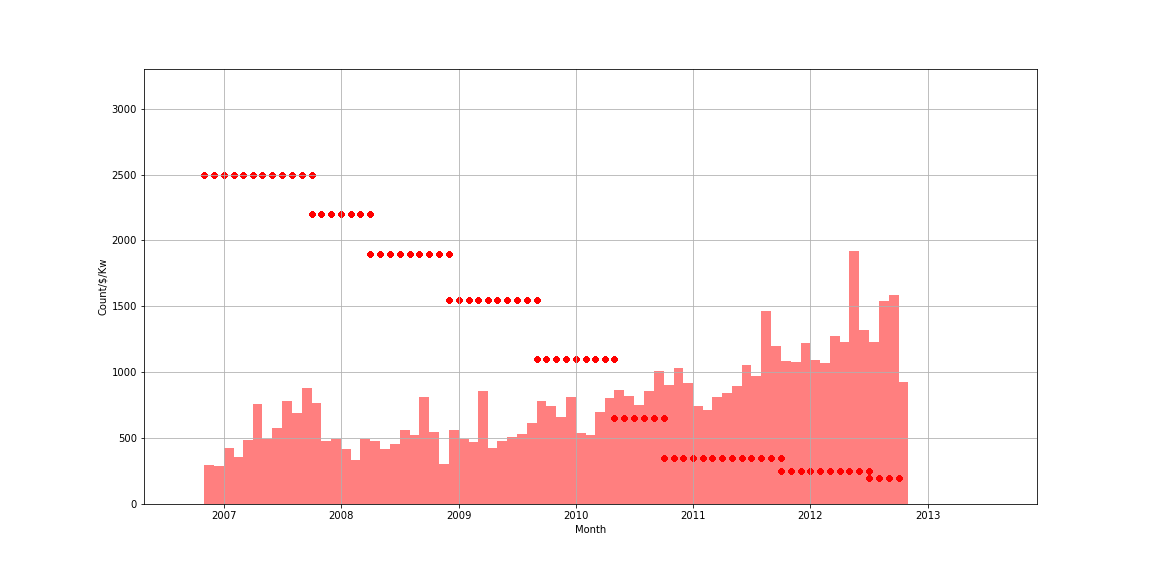
\includegraphics[width = 5in]{app_hist_pge}}\\
\subfloat[SCE]{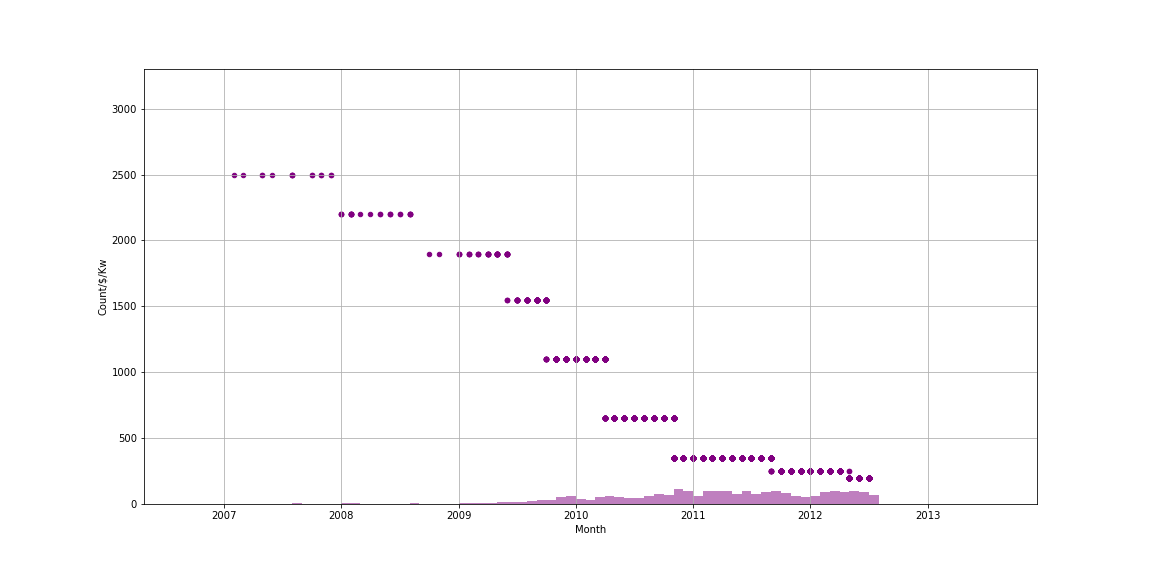
\includegraphics[width = 5in]{app_hist_sdge}}\\
\subfloat[SDGE ]{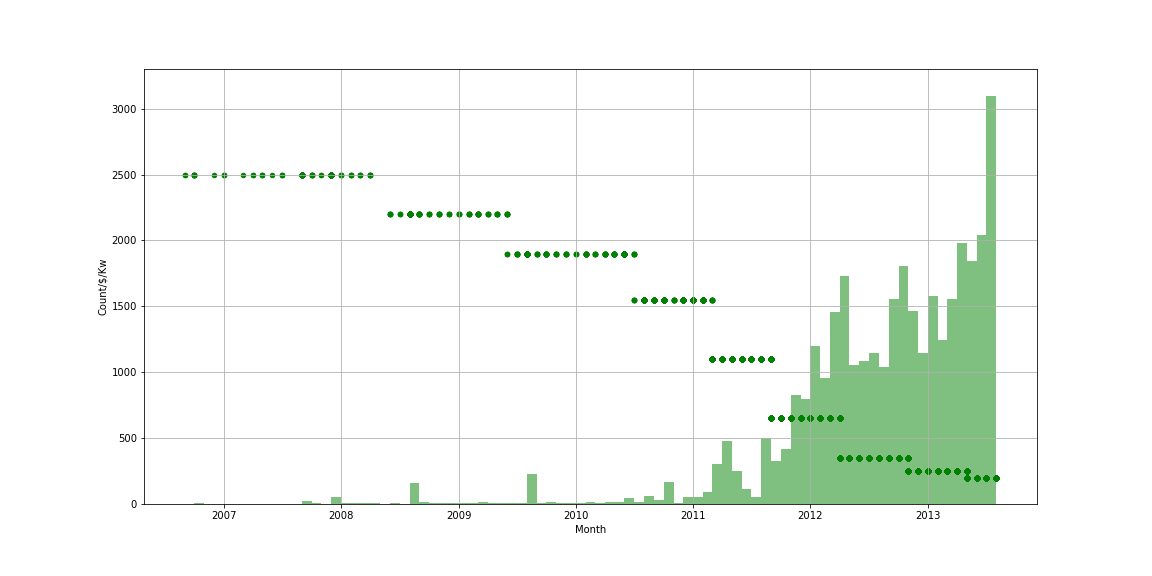
\includegraphics[width = 5in]{app_hist_sce}}\\
\end{tabular}

\end{center}
\caption{The bars are counts of applications received within a month. The dots are subsidy levels during month when applications were received.}
\end{figure}

\begin{thebibliography}{1}

\bibitem{} Branstetter, Lee G. "Are knowledge spillovers international or intranational in scope?: Microeconometric evidence from the US and Japan." Journal of International Economics 53.1 (2001): 53-79.

\bibitem{} Keller, Wolfgang. "Knowledge spillovers at the world's technology frontier." Available at SSRN 271703 (2001).

\bibitem{} Los, Bart, and Bart Verspagen. "R\&D spillovers and productivity: evidence from US manufacturing microdata." Empirical economics 25.1 (2000): 127-148.

\bibitem{} Romer, Paul M. "Increasing returns and long-run growth." Journal of political economy 94.5 (1986): 1002-1037.

\end{thebibliography}

\end{document}